% Définition du répertoire contenant les images
\graphicspath{{IMAGE/}}

% FRAME Intro
\begin{frame}


\includegraphics[width=12cm]{Logos.pdf}

\vfill

\begin{center}

\vspace*{1.5cm}

\LARGE
\textbf{Interaction}

\vspace*{2.5cm}

\large

\textbf{Hadrien Commenges}

{\small

\vspace*{0.1cm}

\url{hadrien.commenges@univ-paris1.fr}}

\end{center}

\end{frame}



% FRAME
\begin{frame}{Cas d'application}

\begin{block}{Interaction}
Mise en relation d'objets géographiques entre eux. Interaction implique que la mise en relation se traduit par une action, uni-, bi- ou multi-directionnelle. Si les objets sont spatialisés, l'interaction a nécessairement une dimension spatiale.
\end{block}

~

La mise en relation peut prendre différentes formes:

\begin{itemize}
\item domaine du vivant: oiseaux migrateurs, réfugiés climatiques, navettes domicile-travail, etc.
\item domaine matériel: échange de marchandises entre pays, échanges sédimentaires dans un cours d'eau, etc.
\item domaine immatériel: jumelage entre communes, amitié Facebook
\end{itemize}


~

\textbf{Quel type d'information géographique est concerné?}

$\rightarrow$ \textit{TYPE 1 - Objets spatialisés}

$\rightarrow$ \textit{TYPE 2 - Occurrences}

\end{frame}



% FRAME
\begin{frame}{Formalisation}

Tout système d'interaction est représentable par une mise en relation d'entités qui prend la forme d'une \textbf{liste de liens} ou d'une \textbf{matrice d'interaction}.

~

La mise en relation peut-être assortie d'un poids (fréquence, volume, etc.)

\begin{figure}
  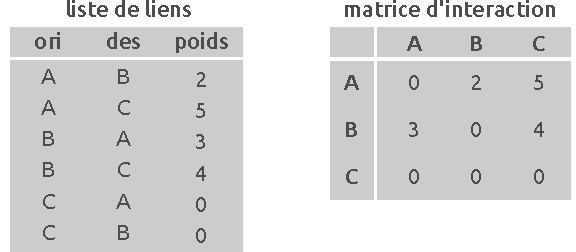
\includegraphics[width=9cm]{MatriceOD.pdf}
\end{figure}

\end{frame}



% FRAME
\begin{frame}{Distance et interaction}

Lorsque l'interaction est spatialisée, elle implique nécessairement une \textbf{distance}.

~

\begin{itemize}
  \item L'interaction spatiale considère \textbf{le déplacement comme un effort}.
  \item L'interaction spatiale est le rapport dialogique entre \textbf{mise en contact} et \textbf{friction de l'éloignement}.
  \item L'interaction spatiale être abordée de deux façons: \textbf{relations entre lieux}  ou \textbf{attraction/influence d'un lieu sur les autres lieux}. 
  \item Dans le premier cas on parlera d'\textbf{analyse de flux}
  \item Dans le second cas on parlera d'\textbf{analyse de position} \\ (\texttt{cf. Accessibilité})
\end{itemize}

\end{frame}


% FRAME
\begin{frame}{Qu'est-ce qu'une distance?}


\textbf{En géographie}, le terme distance désigne une séparation qui demande un effort pour être franchie. La distance est une \textbf{friction}:

\begin{itemize}
  \item ``Everything is related to everything else, but near things are more related than distant things'' (Tobler)
\end{itemize}

~ 

\textbf{En mathématiques}, une distance satisfait les critères suivants:

\begin{itemize}
  \item Symétrie: $d(a, b) = d(b,a)$
  \item Séparation: $d(a, b) = 0 \Longleftrightarrow a = b$
  \item Inégalité triangulaire: $d(a,c) \leq d(a,b) + d(b,c)$
\end{itemize}

\end{frame}


% FRAME
\begin{frame}{Distance euclidienne}

\textbf{Pour un vecteur de dimension 2 (coordonnées x et y):}

\begin{figure}
  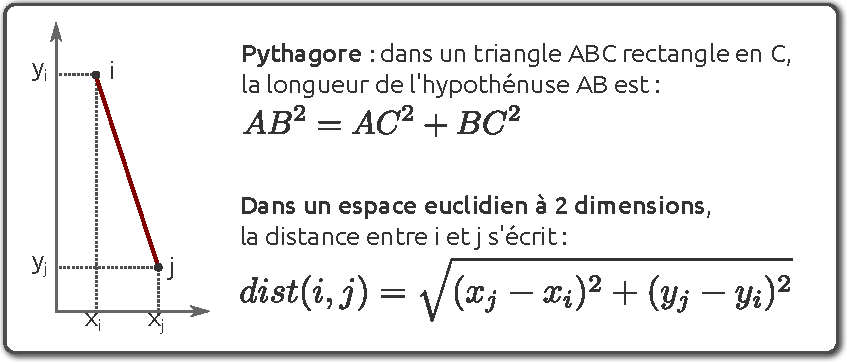
\includegraphics[width=9cm]{DistancesEucli.pdf}
\end{figure}

\textbf{Pour vecteur de dimension $n$:}

\begin{equation}
  \nonumber
  d(a,b) = \sqrt{\sum_{i=1}^n (a_i - b_i)^2}
\end{equation}

\end{frame}


% FRAME
\begin{frame}{Distance de Manhattan}

\textbf{Pour un vecteur de dimension 2:}

\begin{figure}
  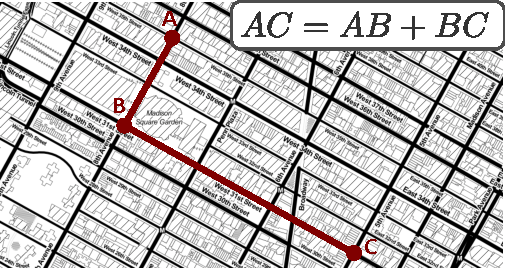
\includegraphics[width=8cm]{DistancesMan.pdf}
\end{figure}

\textbf{Pour vecteur de dimension $n$:}

\begin{equation}
  \nonumber
  d(a,b) = \sum_{i=1}^n |a_i - b_i|
\end{equation}

\end{frame}


% FRAME
\begin{frame}{Distance-réseau, distance-temps, coût généralisé}

\begin{itemize}
  \item \textbf{Distance-réseau:} distance calculée sur un réseau de transport. \\ \textbf{Ex.} Distance calculée sur un réseau en damier (Manhattan).
  \item \textbf{Distance-temps:} éloignement mesuré en temps. Demande de faire un calcul sur le réseau sachant la distance-réseau et la vitesse de déplacement sur ce réseau.
  \item \textbf{Coût généralisé:} quantité composite de temps, d'argent, de confort. Très utilisé en économie des transport.
\end{itemize}

~

$\rightarrow$ les notions de \textbf{distance-réseau} et de \textbf{distance-temps} sont abusives, ces distances satisfont rarement l'\textbf{inégalité triangulaire}.

\end{frame}


% FRAME
\begin{frame}{Distance-réseau, distance-temps, coût généralisé}

\begin{figure}
  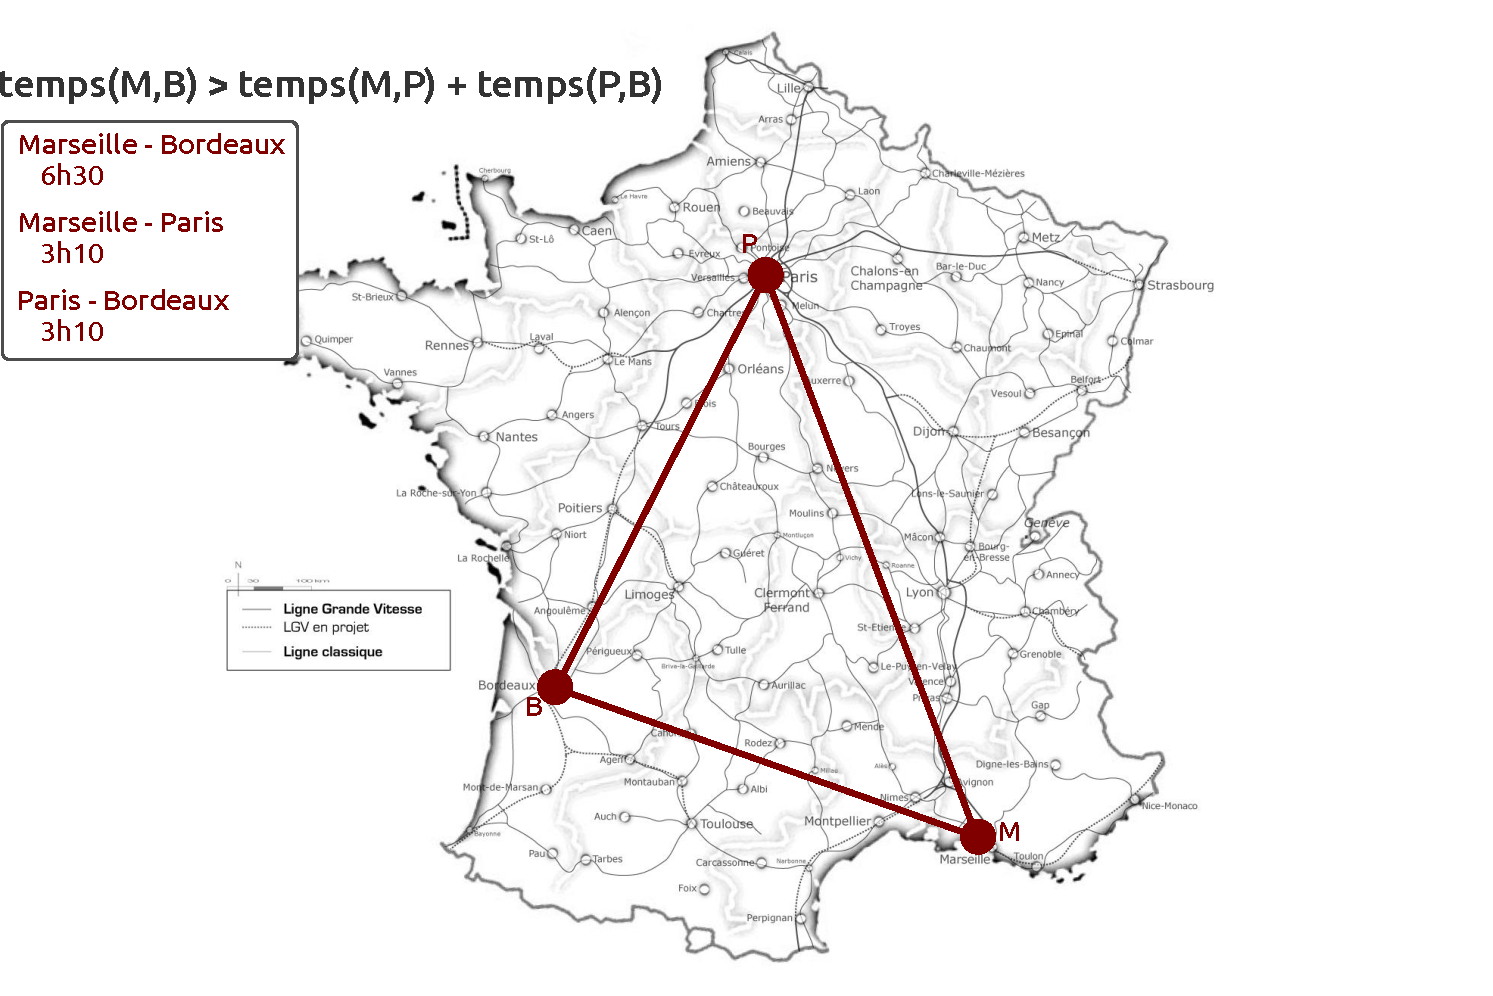
\includegraphics[width=9.8cm]{DistancesTemps.pdf}
\end{figure}

\end{frame}




% FRAME
\begin{frame}{Approches de l'interaction}

\textbf{Trois approches principales:}

\begin{enumerate}
  \item Analyse descriptives des flux observés
  \item Modélisation statistiques des flux
  \item Analyse de graphe, à visée descriptive ou modélisatrice
\end{enumerate}

\end{frame}




% FRAME
\begin{frame}{Analyse de flux: données}

Deux façons de mettre en forme les données: \textbf{format long} (liste de liens) et \textbf{format large} (matrice d'interaction):

~

\begin{figure}
  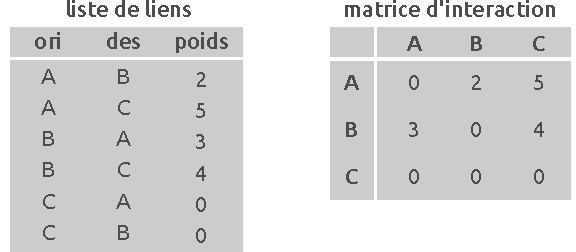
\includegraphics[width=9.5cm]{MatriceOD.pdf}
\end{figure}

\end{frame}


% FRAME
\begin{frame}{Analyse de flux: données}

\begin{figure}
  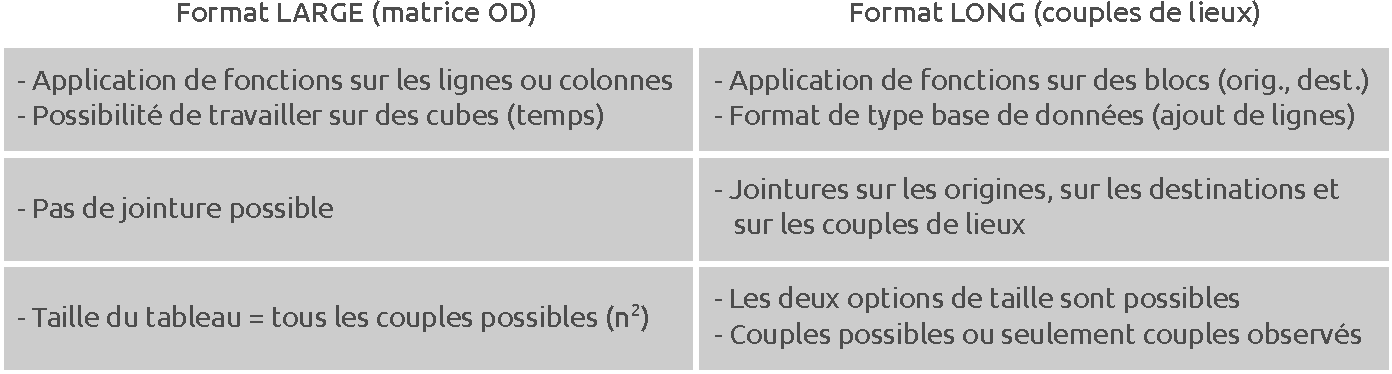
\includegraphics[width=12.1cm]{LongLarge.pdf}
\end{figure}

\begin{block}{La taille compte!}
  \textbf{Plus le maillage est fin, plus la matrice est vide.} \\ \textbf{Ex.:} Navettes domicile-travail, France métropolitaine au RP 2010 \\ \textbf{1,3 milliards} de couples possibles ($36000^2$) et \textbf{1 million} de couples observés: la matrice est \textbf{vide à 99,9\%}.
\end{block}

\end{frame}


% FRAME
\begin{frame}{Analyse de flux: marges}

\begin{itemize}
  \item Les \textbf{sommes marginales} donnent le poids des unités spatiales dans leur rôle d'\textbf{émission} et d'\textbf{attraction}
  \item Le calcul est différent selon le format long ou large des données
\end{itemize}

\begin{figure}
  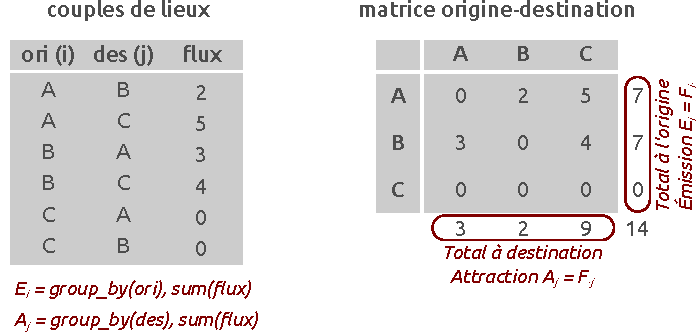
\includegraphics[width=9.5cm]{MatriceOD_marges.pdf}
\end{figure}

\end{frame}



% FRAME
\begin{frame}{Analyse de flux: soldes}

Soldes bruts et relatifs, sur les unités spatiales et sur les flux:

\begin{itemize}
  \item \textbf{Somme (unité spatiales):} $E+A$ 
  \item \textbf{Solde brut (unité spatiales):} $E-A$
  \item \textbf{Solde relatif (unité spatiales):} $(E-A)/(E+A)$ 
  \item \textbf{Somme (flux):} $F_{ij} + F_{ji}$
  \item \textbf{Solde brut (flux):} $F_{ij} - F_{ji}$
  \item \textbf{Solde relatif (flux):} $(F_{ij} - F_{ji}) / (F_{ij} + F_{ji})$
\end{itemize}

~

Deux mesures spécifiques pour les navettes domicile-travail:

\begin{itemize}
  \item \textbf{Autocontention:} $F_{ii} / F_{i \cdot}$
  \item \textbf{Autosuffisance:} $F_{ii} / F_{\cdot j}$
\end{itemize}

\end{frame}


% FRAME
\begin{frame}{Analyse de flux: exploration}

\textbf{Explorer une matrice de flux} consiste à explorer 

\begin{enumerate}
\item les flux
\item les marges
\item les soldes
\end{enumerate}

~ 

avec \ldots

~
\begin{itemize}
  \item \ldots des mesures de centralité et de dispersion
  \item \ldots des graphiques (histogrammes, boîtes, nuages)
  \item \ldots des cartes (flux et stocks)
\end{itemize}

\end{frame}



% FRAME
\begin{frame}{Modélisation des flux: approches}

\textbf{Historiquement, deux grandes approches ont été proposées:}

\begin{itemize}
  \item \textbf{Gravitation:} racines au 19e siècle (Casey, Ravenstein), appliqué par Reilly (1931), informatisé dans les années 1950 (USA, transport). Massivement utilisé dans plusieurs domaines (transport, géographie, démographie, économie).
  \item \textbf{Interposition:} proposé par Stouffer (1942) informatisé dans les années 1950 (USA, transport), informatisé dans les années 1950 (USA, transport). Assez peu utilisé jusqu'à ce jour, repris récemment sous le nom de \textbf{radiation}.
\end{itemize}

\end{frame}


% FRAME
\begin{frame}{Modélisation des flux: approches}

\textbf{La mise en place d'un modèle d'interaction spatiale passe par trois étapes de formalisation:}

\begin{enumerate}
  \item \textbf{Formalisation conceptuelle} des entités (individus, unités spatiales) et des relations (échanges d'individus, de biens, d'informations).
  \item \textbf{Formalisation mathématique} qui définit la nature et l'intensité des interactions dans un jeu d'équations.
  \item \textbf{Formalisation informatique} qui implémente les équations dans un langage de programmation.
\end{enumerate}



\end{frame}



% FRAME
\begin{frame}{Modélisation des flux: formalisation}

\textbf{Le modèle gravitaire d'origine s'écrit:}

\begin{equation}
\nonumber
T_{ij} = k \frac{P_i P_j}{D_{ij}^{2}}
\end{equation}

~

De nombreuses versions existent qui n'ont plus grand' chose à voir avec la loi de gravité newtonienne. On jour principalement sur:

\begin{itemize}
  \item \textbf{Nature des masses:} populations, emplois, émissions, attractions
  \item \textbf{Pondération des masses:} paramètres multiplicateurs ou exposants
  \item \textbf{Fonction de friction:} puissance négative, exponentielle  négative
  \item \textbf{Contraintes aux marges:} contrainte double, simple, absente
  \item \textbf{Résolution numérique} du système
\end{itemize}


\end{frame}


% FRAME
\begin{frame}{Modélisation des flux: formalisation}

\textbf{Le modèle d'opportunités interposées} (Stouffer 1960) s'écrit:

\begin{equation}
\nonumber
T_{ij} = k_i O_i \left[\exp(-\alpha x_{j-1}) - \exp(-\alpha x_{j}) \right]
\end{equation}

~

\textbf{Le modèle de radiation} (Simini \textit{et al.} 2012) s'écrit:  

\begin{figure}
  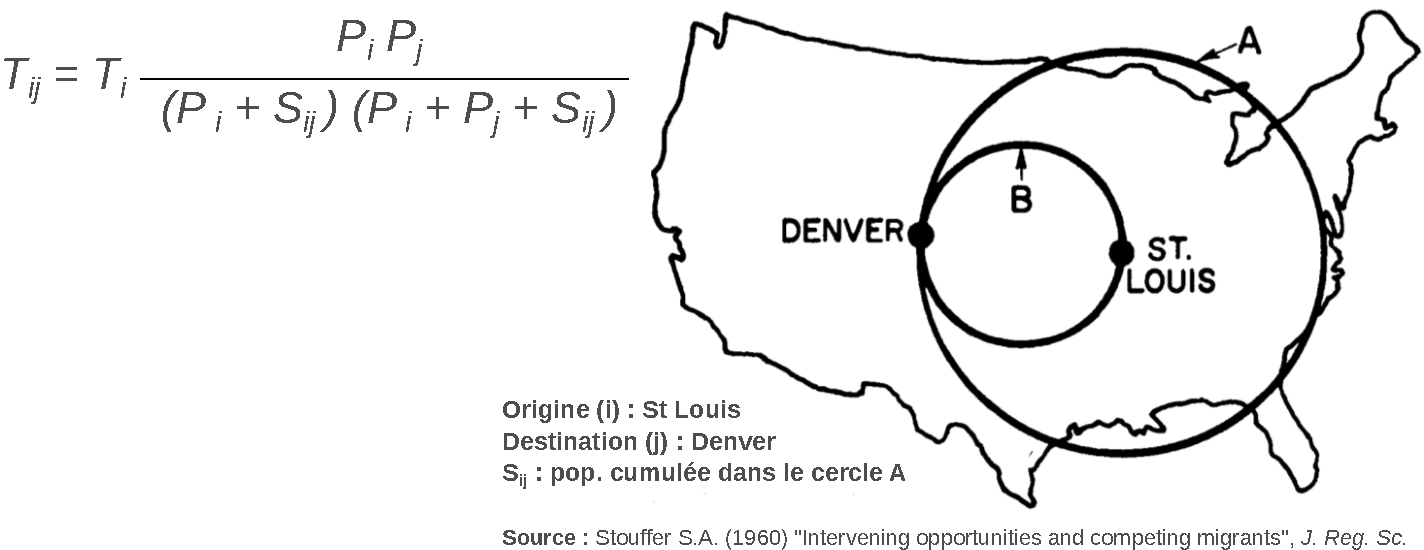
\includegraphics[width = 110mm]{CercleStouffer.pdf}
\end{figure}

\end{frame}


% FRAME
\begin{frame}{Analyse de graphe}

Leonhard Euler et \textbf{les sept ponts de Koenigsberg} (Kaliningrad).


\begin{figure}
  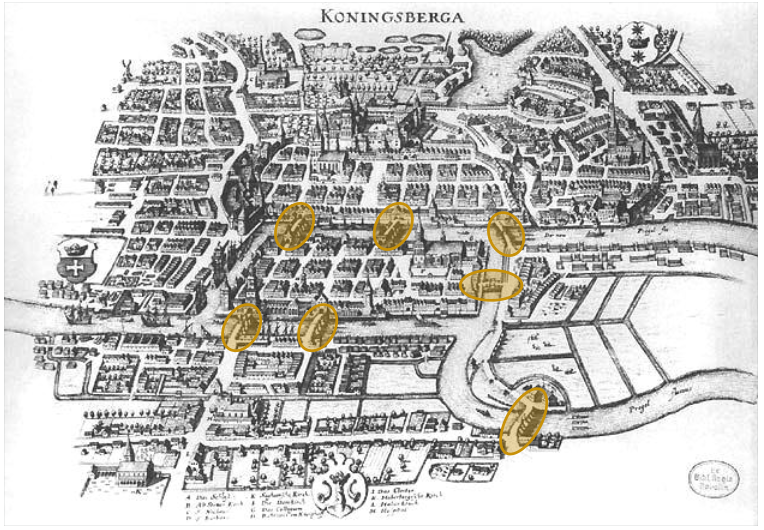
\includegraphics[width=10cm]{Konigsberg.png}
\end{figure}

\end{frame}


% FRAME
\begin{frame}{Analyse de graphe}

\begin{figure}
  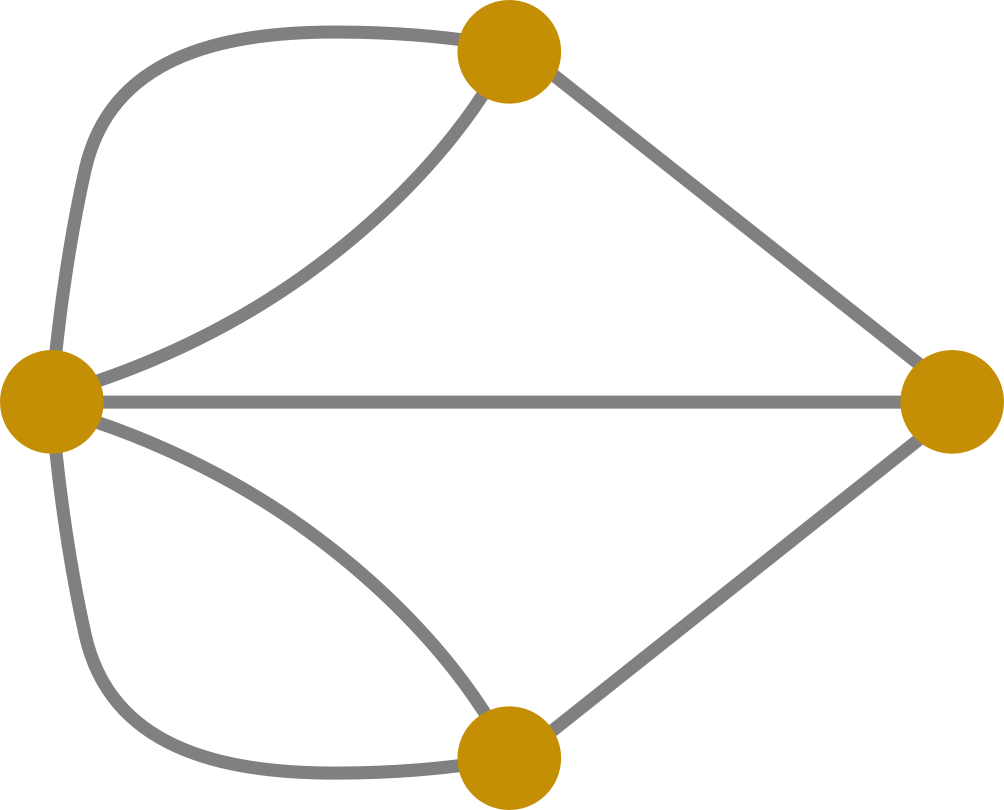
\includegraphics[width=5cm]{Konigsberg_graph.png}
\end{figure}

~

\begin{itemize}
\item Pas de \textbf{cycle eulérien} (parité des liens incidents)
\item Pas de \textbf{chaîne eulérienne} (continuité du tracé)
\end{itemize}


\end{frame}



% FRAME
\begin{frame}{Réseau social}

\begin{figure}
  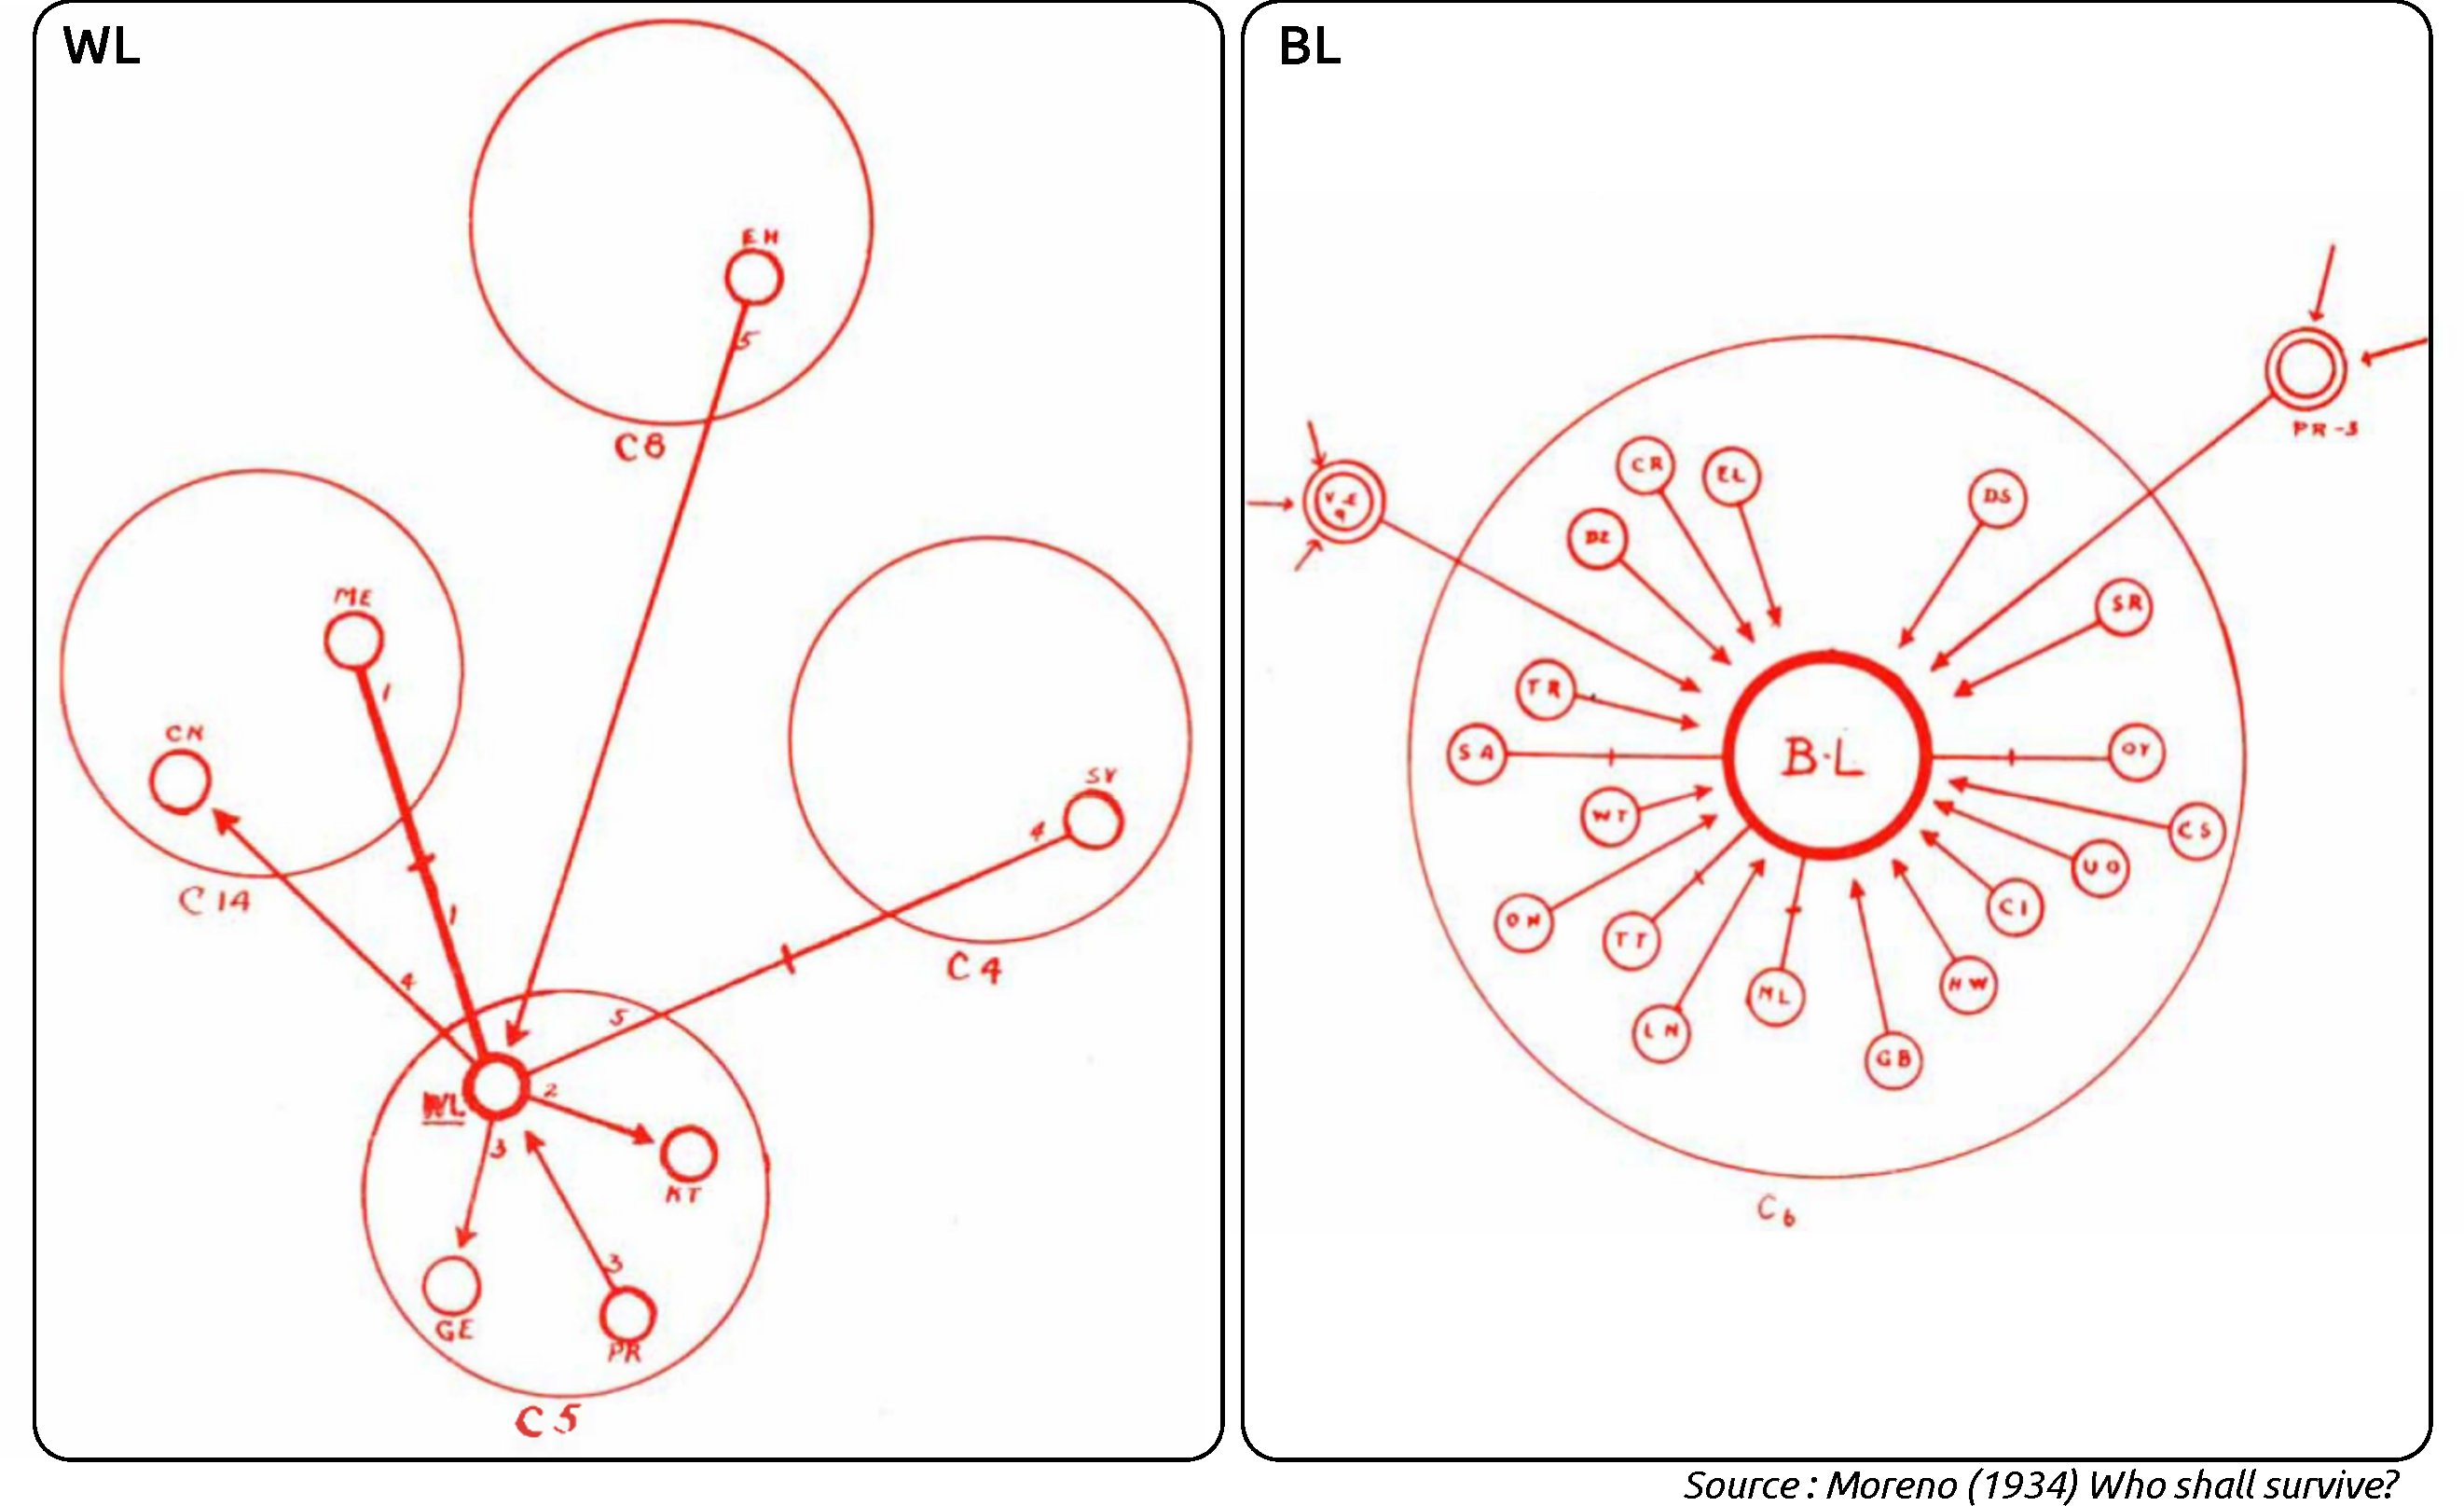
\includegraphics[width=12cm]{Moreno.pdf}
\end{figure}

\end{frame}


% FRAME
\begin{frame}{Qu'est-ce qu'un graphe?}

Les graphes sont des objets mathématiques composés de \textbf{sommets} (n{\oe}ds, \textit{vertices}) et de \textbf{liens} (arcs, \textit{edges}). Ils représentent des objets divers:

\begin{itemize} 
  \item \textbf{Réseaux de transport:} métro modélisé avec des stations (n{\oe}uds) et des lignes (arcs)
  \item \textbf{Réseaux sociaux:} réseau \textit{facebook} avec des individus (n{\oe}uds) et liens d'amitié (arcs)
  \item \textbf{Réseaux bibliométriques:} réseau de chercheurs (n{\oe}uds) et reliés par des liens de co-publication (arcs)
  \item \ldots
\end{itemize}

\end{frame}



% FRAME
\begin{frame}{Types de graphes}

\textbf{Graphe orienté et valué:}

\begin{figure}
  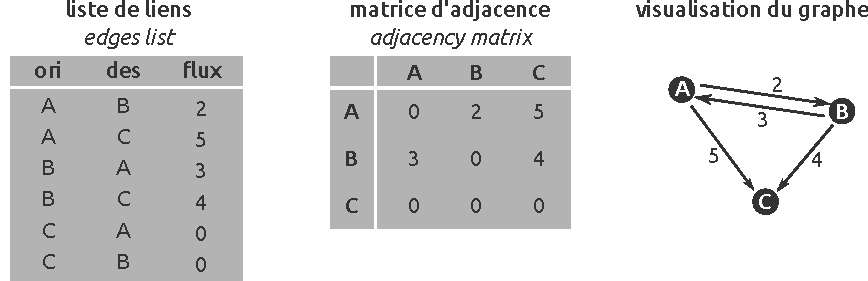
\includegraphics[width=12cm]{MatGraph1.pdf}
\end{figure}

\end{frame}


% FRAME
\begin{frame}{Types de graphes}

\textbf{Graphe orienté et non-valué:}

\begin{figure}
  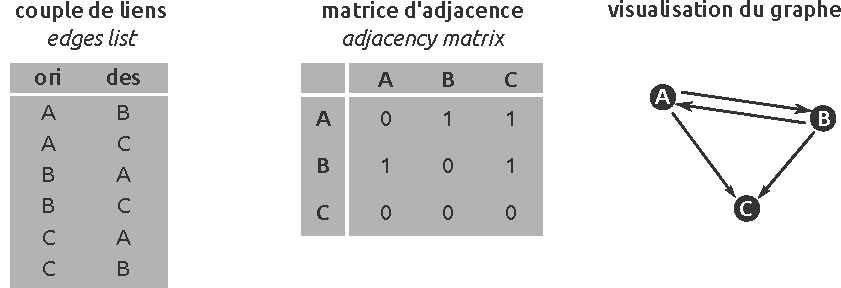
\includegraphics[width=12cm]{MatGraph2.pdf}
\end{figure}

\end{frame}


% FRAME
\begin{frame}{Types de graphes}

\textbf{Graphe non-orienté et non-valué:}

\begin{figure}
  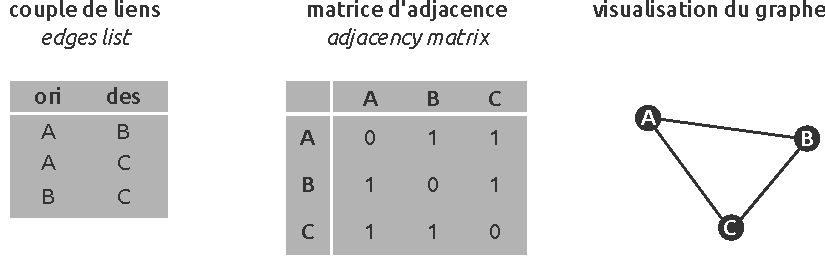
\includegraphics[width=12cm]{MatGraph3.pdf}
\end{figure}

\end{frame}



% FRAME
\begin{frame}{Principales mesures descriptives}

\textbf{Mesures globales:}

\begin{itemize}
\item nombre de noeuds
\item nombre d’arcs
\item nombre de composantes connexes
\item rapport entre nombre d’arcs et nombre de noeuds (densité)
\item diamètre du graphe: longueur du plus long des plus courts chemins
\item rapport entre nombre d’arcs et nombre maximum d’arcs (connectivité)
\end{itemize}

~

$\rightarrow$ \textbf{Nombre maximum d’arcs (sans boucle):}

\begin{itemize}
\item pour un graphe planaire: $3V - 6$
\item pour un graphe non planaire non orienté: $\frac{V(V-1)}{2}$ 
\item pour un graphe non planaire orienté: $V(V-1)$
\end{itemize}

\end{frame}

% FRAME
\begin{frame}{Principales mesures descriptives}

\textbf{Mesures locales de centralité:}

\begin{itemize}
\item Degré: nombre d'arcs incidents (nbr. de voisins)
\item Degré pondéré: nbr. d’arcs incidents pondérés
\item Centralité de proximité (\textit{closeness}): inverse de la somme des distances à tous les autres noeuds
\item Centralité d'intermédiarité (\textit{betweenness}): nombre de plus courts chemins passant par un noeud (standardisé)
\end{itemize}


\end{frame}
